\chapter{Introduction}

In this tutorial we will see some basic concepts of deductive program verification of C programs. We will use a tool called Frama-C\footnote{\url{https://www.frama-c.com}} (FRAmework for Modular Analysis of C code), and its specification language ACSL (ANSI C Specification Language). ACSL annotations can however also be used by tools other than Frama-C, such as the model checker TriCera \cite{esen2022tricera} developed at Uppsala University. 

Frama-C is actually not a single tool, but a collection of different code analysis tools. It provides a common interface for different \emph{plugins} performing different analyses on the code we provide. Here is an overview of the plugins available in the standard Frama-C distribution:

\begin{center}
    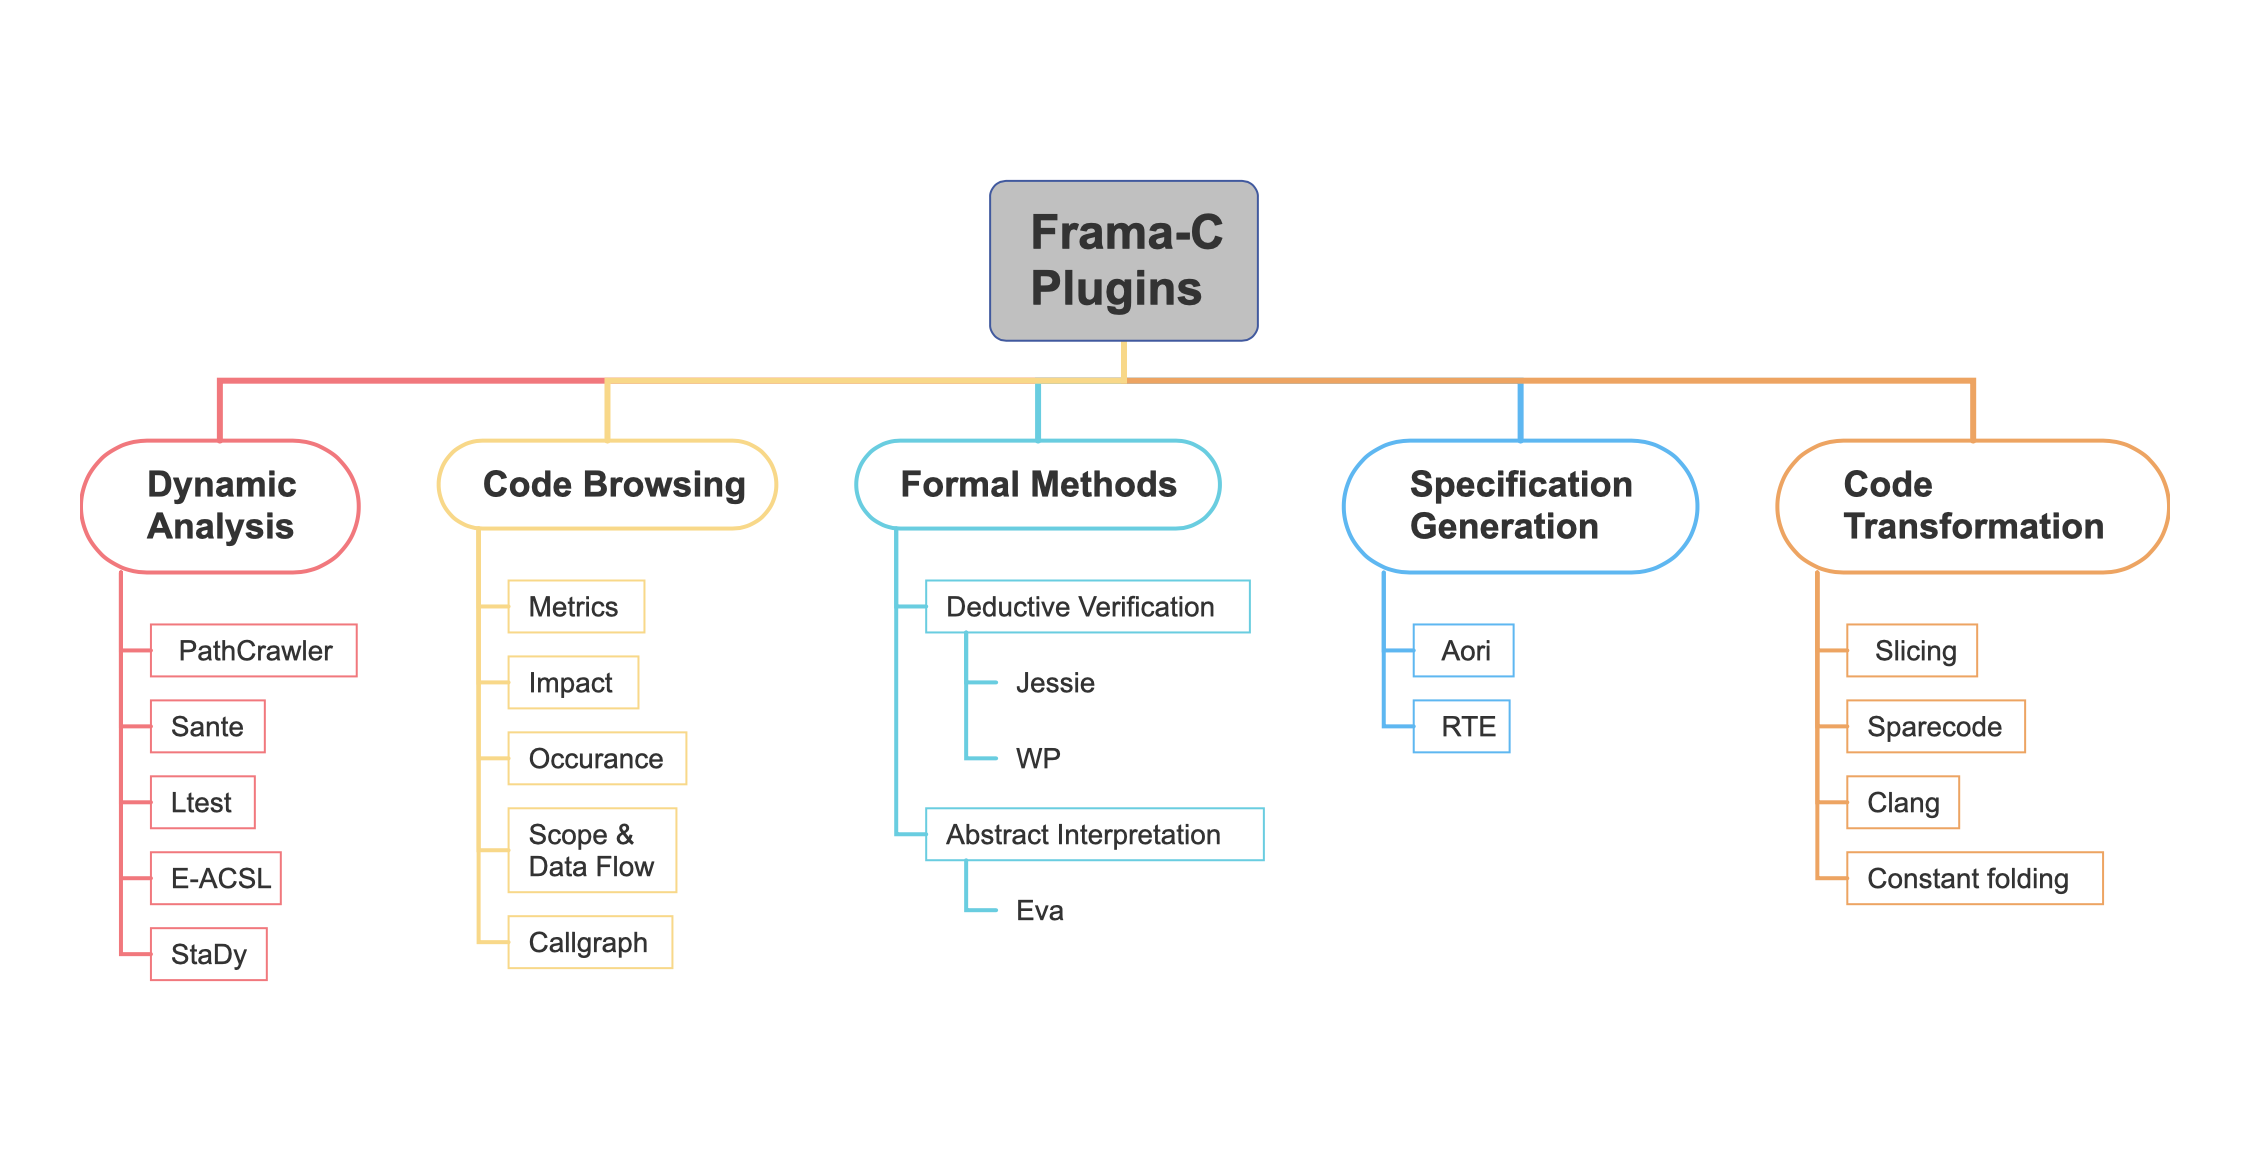
\includegraphics[width=\textwidth]{images/frama_c_plugins.png}
\end{center}

In this tutorial we will only use the WP plugin, which performs deductive verification on our C code. WP stands for \emph{weakest precondition}, a theory we have seen during the verification lecture that builds the basis of this plugin. We will however not look deeper into the theory, and only see how we can use Frama-C in practice for proving properties of our programs. 

This introduction barely scratches the surface of what is possible with Frama-C. It shall just give you an idea of the power of static program verification, and hopefully inspire you to look deeper on your own. 

While this text is mostly self-contained, I would like to mention a few resources that can come in handy if you should ever find yourself stuck, or you would like to gain some deeper insight into some of the provided functionality. 

The first important resource is the manual of Frama-C itself \cite{correnson_frama-c_nodate}. ACSL has its own seperate manual \cite{baudin_acsl_nodate}. A sightly more complex, but also more thorough introduction into Frama-C and ACSL can be found in \cite{prevosto_acsl_nodate}. 

In \cite{blanchard_introduction_2020} the author gives a tutorial that covers almost everything ACSL offers. It is very approachable, and might be a good starting point after working through this tutorial. Last but not least, \cite{gerlach_acsl_2020} tries to teach ACSL through examples by going through the verification of many algorithms that are part of the C++ standard library. 
